\documentclass[aps,english,prb,floatfix,amsmath,superscriptaddress,tightenlines,twocolumn,nofootinbib]{revtex4-2}
\usepackage{mathtools, amssymb}
\usepackage{tikz}
\usepackage{tikz-3dplot}
\usetikzlibrary{spy}
\usetikzlibrary{arrows.meta}
\usetikzlibrary{calc}
\usetikzlibrary{decorations.pathreplacing,calligraphy}
\usepackage[utf8]{inputenc}
\usepackage{xcolor}
\usepackage{tcolorbox}

\begin{document}

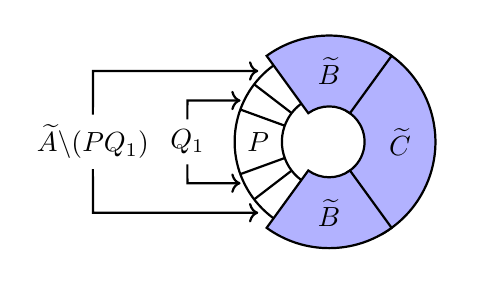
\begin{tikzpicture}[every path/.style={thick}, scale=0.6]
    \draw[] (120:1cm) -- (120:2cm) -- (120:2cm) arc (120:240:2cm) -- (240:1cm) -- (240:1cm) arc (240:120:1cm) -- cycle;
    \draw[fill=blue!30!white] (60:0.75cm) -- (60:2.25cm) -- (60:2.25cm) arc (60:-60:2.25cm) -- (-60:0.75cm) -- (-60:0.75cm) arc (-60:60:0.75cm) -- cycle;
    \draw[fill=blue!30!white] (54:0.75cm) -- (54:2.25cm) -- (54:2.25cm) arc (54:126:2.25cm) -- (126:0.75cm) -- (126:0.75cm) arc (126:54:0.75cm) -- cycle;
    \draw[fill=blue!30!white] (-54:0.75cm) -- (-54:2.25cm) -- (-54:2.25cm) arc (-54:-126:2.25cm) -- (-126:0.75cm) -- (-126:0.75cm) arc (-126:-54:0.75cm) -- cycle;
  
    \draw[] (160:1cm) -- (160:2cm);
    \draw[] (200:1cm) -- (200:2cm);

    \draw[] (142.5:1cm) -- (142.5:2cm);
    \draw[] (217.5:1cm) -- (217.5:2cm);
    
    \node[] () at (180:1.5cm) {$P$};
    \node[] () at (0:1.5cm) {$\widetilde{C}$};
    \node[] () at (90:1.5cm) {$\widetilde{B}$};
    \node[] () at (-90:1.5cm) {$\widetilde{B}$};
    \node[] (sub) at (-5cm,0) {$\widetilde{A}{\setminus}(PQ_1)$};
    \node[] (q1) at (-3cm, 0) {$Q_1$};

    \draw[->] (q1) -- (-3, 0.875) -- (-1.875, 0.875);
    \draw[->] (q1) -- (-3, -0.875) -- (-1.875, -0.875);

    \draw[->] (sub) -- (-5, 1.5) -- (-1.5, 1.5);
    \draw[->] (sub) -- (-5, -1.5) -- (-1.5, -1.5);
    \end{tikzpicture}

\end{document}